\chap{ An Enhanced Processor}

\section{Part 3}
In this part you will extend the capability of the processor so that the external counter is no longer needed, and so
that the processor has the ability to perform read and write operations using memory or other devices. You will
add three new types of instructions to the processor, as displayed in Table 3. The ld (load) instruction loads data
into register RX from the external memory address specified in register RY. The st (store) instruction stores the
data contained in register RX into the memory address found in RY. Finally, the instruction mvnz (move if not
zero) allows a mv operation to be executed only under the condition that the current contents of register G are not
equal to 0.\\
\begin{figure}[h]
    \centering
    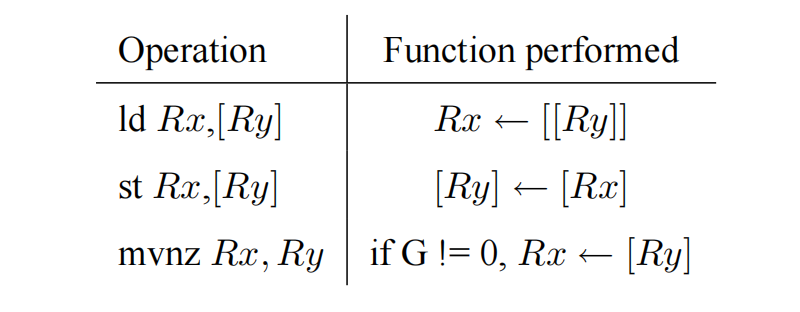
\includegraphics[scale = 0.6]{source/picture/Lab10/pic1.png}
\end{figure}

A schematic of the enhanced processor is given in Figure 11. In this figure, registers R0 to R6 are the same
as in Figure 1 of Laboratory Exercise 9, but register R7 has been changed to a counter. This counter is used
to provide the addresses in the memory from which the processor’s instructions are read; in the preceding lab
exercise, a counter external to the processor was used for this purpose. We will refer to R7 as the processor’s
program counter (PC), because this terminology is common for real processors available in the industry. When
the processor is reset, PC is set to address 0. At the start of each instruction (in time step 0) the contents of PC
are used as an address to read an instruction from the memory. The instruction is stored in IR and the PC is
automatically incremented to point to the next instruction (in the case of mvi the PC provides the address of the
immediate data and is then incremented again).\\
The processor’s control unit increments PC by using the $incr_PC$ signal, which is just an enable on this counter. It
is also possible to directly load an address into PC (R7) by having the processor execute a mv or mvi instruction
in which the destination register is specified as R7. In this case the control unit uses the signal R7in to perform
a parallel load of the counter. In this way, the processor can execute instructions at any address in memory, as
opposed to only being able to execute instructions that are stored in successive addresses. Similarly, the current
contents of PC can be copied into another register by using a mv instruction. An example of code that uses the
PC register to implement a loop is shown below, where the text after the \% on each line is just a comment. The
instruction mv R5,R7 places into R5 the address in memory of the instruction sub R4,R2. Then, the instruction
mvnz R7,R5 causes the sub instruction to be executed repeatedly until R4 becomes 0. This type of loop could be
used in a larger program as a way of creating a delay\\
\begin{figure}[h]
    \centering
    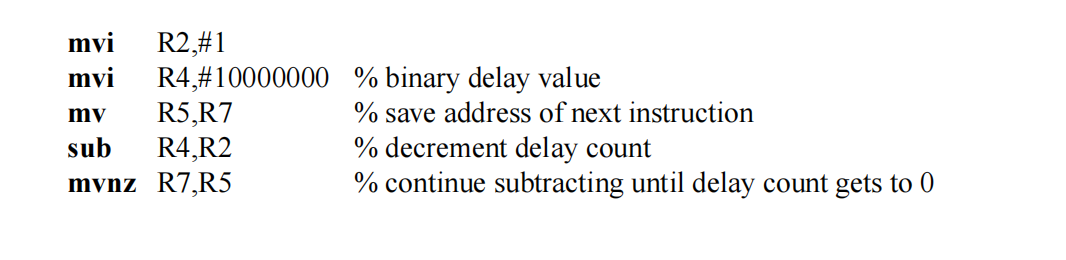
\includegraphics[scale = 0.6]{source/picture/Lab10/pic2.png}
\end{figure}
\newpage
Figure 11 shows two registers in the processor that are used for data transfers. The ADDR register is used to send
addresses to an external device, such as a memory module, and the DOUT register is used by the processor to
provide data that can be stored outside the processor. One use of the ADDR register is for reading, or fetching, instructions from memory; when the processor wants to fetch an instruction, the contents of PC (R7) are transferred
across the bus and loaded into ADDR. This address is provided to memory. In addition to fetching instructions,
the processor can read data at any address by using the ADDR register. Both data and instructions are read into the
processor on the DIN input port. The processor can write data for storage at an external address by placing this
address into the ADDR register, placing the data to be stored into its DOUT register, and asserting the output of
the W (write) flip-flop to 1.\\
Figure 12 illustrates how the enhanced processor is connected to memory and other devices. The memory unit
in the figure supports both read and write operations and therefore has both address and data inputs, as well as a
write enable input. The memory also has a clock input, because the address, data, and write enable inputs must be
loaded into the memory on an active clock edge. This type of memory unit is usually called a synchronous static
random access memory (synchronous SRAM). Figure 12 also includes a 9-bit register that can be used to store data
2
ADDR DOUT
from the processor; this register might be connected to a set of LEDs to allow display of data on your DE-series
board. To allow the processor to select either the memory unit or register when performing a write operation, the
circuit includes some logic gates that perform address decoding: if the upper address lines are A8A7 = 00, then
the memory module will be written at the address given on the lower address lines. Figure 12 shows n lower
address lines connected to the memory; for this exercise a memory with 128 words is probably sufficient, which
implies that n = 7 and the memory address port is driven by A6 . . . A0. For addresses in which A8A7 = 01, the
data written by the processor is loaded into the register whose outputs are called LEDs in Figure 12.\\
\begin{figure}[h]
    \centering
    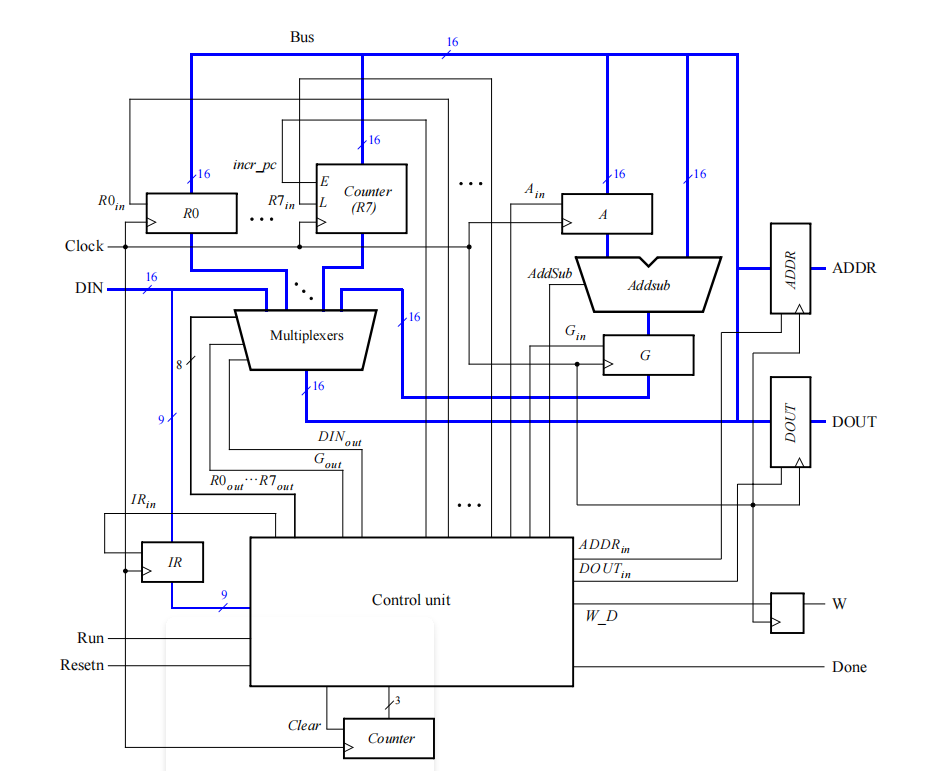
\includegraphics[scale = 0.5]{source/picture/Lab10/pic3.png}
\end{figure}

1. Create a new Quartus project for the enhanced version of the processor.\\
2. Write Verilog code for the processor and test your circuit by using functional simulation: apply instructions
to the DIN port and observe the internal processor signals as the instructions are executed. Pay careful
attention to the timing of signals between your processor and external memory; account for the fact that the
memory has registered input ports, as we discussed for Figure 12.\\
3. Create another Quartus project that instantiates the processor, memory module, and register shown in Figure 12. Use the Quartus IP Catalog to create the RAM: 1-PORT memory module. Follow the instructions
provided by the wizard to create a memory that has one 9-bit wide read/write data port and is 128 words
deep. Ensure that the output is not registered. Use a MIF file to store instructions in the memory that are to
be executed by your processor. An example program in the form of a MIF file is shown in Figure 13. This
program display an 8-bit counter value on the LEDs output port. Loops are used in the program to create
delays so that the counter values are not changed too quickly to be observed. Comments are included in the
MIF file in Figure 13 to describe the program’s code.\\
4. Use functional simulation to test the circuit. Ensure that data is read properly from the memory and executed
by the processor.\\
5. Include in your project the necessary pin assignments to implement your circuit on your DE-series board.
Use switch SW9 to drive the processor’s Run input, use KEY0 for Resetn, and use the board’s 50 MHz
clock signal as the Clock input. Since the circuit needs to run properly at 50 MHz, make sure that a timing
constraint is set in Quartus to constrain the circuit’s clock to this frequency. Read the Report produced
by the Quartus Timing Analyzer to ensure that your circuit operates at this speed; if not, use the Quartus
tools to analyze your circuit and modify your Verilog code to make a more efficient design that meets the
3
Resetn
Run
50-MHz speed requirement. Also note that the Run input is asynchronous to the clock signal, so make sure
to synchronize this input using flip-flops.\\
Connect the LEDs register in Figure 12 to $LEDR_{8-0}$ so that you can observe the output produced by the
processor\\
\newpage
\lstdefinestyle{verilog-style}
{
    language=Verilog,
    basicstyle=\small\ttfamily,
    keywordstyle=\color{vblue},
    identifierstyle=\color{black},
    commentstyle=\color{vgreen},
    numbers=left,
    numberstyle=\tiny\color{black},
    numbersep=10pt,
    tabsize=8,
    moredelim=*[s][\colorIndex]{[}{]},
    literate=*{:}{:}1
}
\definecolor{vgreen}{RGB}{104,180,104}
\definecolor{vblue}{RGB}{49,49,255}
\definecolor{vorange}{RGB}{255,143,102}

\makeatletter
\newcommand*\@lbracket{[}
\newcommand*\@rbracket{]}
\newcommand*\@colon{:}
\newcommand*\colorIndex{%
    \edef\@temp{\the\lst@token}%
    \ifx\@temp\@lbracket \color{black}%
    \else\ifx\@temp\@rbracket \color{black}%
    \else\ifx\@temp\@colon \color{black}%
    \else \color{vorange}%
    \fi\fi\fi
}
\makeatother


\subsection{Code, memory and Simulation}
\begin{lstlisting}[style={verilog-style}]
module part3 ( W,BusWires,ADDR,SW, KEY, LEDR,Tstep ,EN,Done);  //Main part Run
  # Initial Variable
  input EN;
  input [8:0] SW;
  input [2:0] KEY;
  output reg [8:0] LEDR;
  output [2:0] Tstep;
  output Done;
  wire [8:0] DIN, DOUT, LEDsOUT;
  wire Resetn, Clock, Run;
  output W;
  output [8:0]BusWires,ADDR;
  reg LEDen, MEMen;

  assign MClock = KEY[1];
  assign PClock = KEY[2];

  assign Resetn = KEY[0];
  
  wire [8:0] R0;
  always
    if (EN)
      LEDR[8:0] = DIN;
    else
      LEDR[8:0] = R0;
  
  always
  begin
    LEDen = W & ~( ADDR[8] | ~ADDR[7]);
    MEMen = W & ~( ADDR[8] | ADDR[7]);
  end
  
  proc P0 (DIN, Resetn, PClock, Run, Done, BusWires, ADDR, DOUT, W, Tstep[2:0], R0);
  regn LEDs (DOUT, LEDen, MClock, LEDsOUT);
  Me Memory (ADDR, MClock, DOUT, MEMen, DIN);

endmodule

//The main processor
module processor (DIN, Resetn, Clock, Run, Done, BusWires, ADDR,
DOUT, W, Tstep_Q, R0);
  input [8:0] DIN;
  input Resetn, Clock, Run;
  output reg Done;
  output reg [8:0] BusWires;
  output [8:0] ADDR, DOUT;
  output W;
  output [2:0] Tstep_Q;
  output [8:0] R0;
 // output [8:0] A, G;
  //declare variables
  reg IRin, DINout, Ain, Gout, Gin, AddSub, incr_pc, ADDRin, DOUTin, W_D;
  reg [7:0] Rout, Rin;
  wire [7:0] Xreg, Yreg;
  wire [1:9] IR;
  wire [1:3] I;
  reg [9:0] MUXsel;
  wire [8:0] R0, R1, R2, R3, R4, R5, R6, R7, result;
  wire [8:0] A, G;
  wire [2:0] Tstep_Q;

  wire Clear = Done | ~Resetn;
  upcount Tstep (Clear, Clock, Tstep_Q);
  assign I = IR[1:3];
  dec3to8 decX (IR[4:6], 1'b1, Xreg);
  dec3to8 decY (IR[7:9], 1'b1, Yreg);
  always @(Tstep_Q or I or Xreg or Yreg)
  begin
    //specify initial values
    IRin = 1'b0;
    Rout[7:0] = 8'b00000000;
    Rin[7:0] = 8'b00000000;
    DINout = 1'b0;
    Ain = 1'b0;
    Gout = 1'b0;
    Gin = 1'b0;
    AddSub = 1'b0;
    DOUTin = 1'b0;
    ADDRin = 1'b0;
    W_D = 1'b0;
    incr_pc = 1'b0;

    Done = 1'b0;

    case (Tstep_Q)
      3'b000: // load next instruction in time step 0
      begin
        Rout = 8'b00000001;
        ADDRin = 1'b1;
        incr_pc = 1'b1;
		  IRin = 1'b1;
      end
      3'b001: //define signals in time step 1
        case (I)
          3'b000: // mv
          begin
            Rout = Yreg;
            Rin = Xreg;
            Done = 1'b1;
          end
          3'b001: // mvi
          begin
            DINout = 1'b1;
            Rin = Xreg;
            Done = 1'b1;
            incr_pc = 1'b1;
          end
          3'b010: // add
          begin
            Rout = Xreg;
            Ain = 1'b1;
          end
          3'b011: // sub
          begin
            Rout = Xreg;
            Ain = 1'b1;
          end
          3'b100: // ld
          begin
            Rout = Yreg;
            ADDRin = 1'b1;
          end
          3'b101: // st
          begin
            Rout = Xreg;
            DOUTin = 1'b1;
          end
          3'b110: // mvnz
          begin
            if (G != 0) begin
              Rout = Yreg;
              Rin = Xreg;
            end
            Done = 1'b1;
          end
        endcase
      3'b010: //define signals in time step 2
        case (I)
          3'b010: // add
          begin
            Rout = Yreg;
            Gin = 1'b1;
				AddSub = 1'b1;
          end
          3'b011: // sub
          begin
            Rout = Yreg;
            Gin = 1'b1;
            AddSub = 1'b1;
          end
          3'b100: // ld
          begin
            DINout = 1'b1;
            Rin = Xreg;
            Done = 1'b1;
          end
          3'b101: // st
          begin
            Rout = Yreg;
            ADDRin = 1'b1;
            W_D = 1'b1;
				//Done = 1'b1;
          end
        endcase
      3'b011: //define signals in time step 3
        case (I)
          3'b010: // add
          begin
            Gout = 1'b1;
            Rin = Xreg;
            Done = 1'b1;
          end
          3'b011: // sub
          begin
            Gout = 1'b1;
            Rin = Xreg;
            Done = 1'b1;
          end
        endcase
    endcase
  end

  //instantiate registers and the adder/subtracter unit

  counter reg_0 (1'b1, Clock, incr_pc, BusWires, ~Resetn, Rin[0], R0);
  regn reg_1 (BusWires, Rin[1], Clock, R1);
  regn reg_2 (BusWires, Rin[2], Clock, R2);
  regn reg_3 (BusWires, Rin[3], Clock, R3);
  regn reg_4 (BusWires, Rin[4], Clock, R4);
  regn reg_5 (BusWires, Rin[5], Clock, R5);
  regn reg_6 (BusWires, Rin[6], Clock, R6);
  regn reg_7 (BusWires, Rin[7], Clock, R7);

  regn reg_IR (DIN, IRin, Clock, IR);
  defparam reg_IR.n = 9;
  regn reg_A (BusWires, Ain, Clock, A);
  regn reg_G (result, Gin, Clock, G);

  regn reg_ADDR (BusWires, ADDRin, Clock, ADDR);
  regn reg_DOUT (BusWires, DOUTin, Clock, DOUT);
  regn reg_W (W_D, 1'b1, Clock, W);
  defparam reg_W.n = 1; 

  add_sub AS (~AddSub, A, BusWires, result);

  //define the bus
  always @ (MUXsel or Rout or Gout or DINout)
  begin
    MUXsel[9:2] = Rout;
    MUXsel[1] = Gout;
    MUXsel[0] = DINout;
    
    case (MUXsel)
      10'b0000000001: BusWires = DIN;
      10'b0000000010: BusWires = G;
      10'b0000000100: BusWires = R0;
      10'b0000001000: BusWires = R1;
      10'b0000010000: BusWires = R2;
      10'b0000100000: BusWires = R3;
      10'b0001000000: BusWires = R4;
      10'b0010000000: BusWires = R5;
      10'b0100000000: BusWires = R6;
      10'b1000000000: BusWires = R7;
    endcase
  end

endmodule


module upcount(Clear, Clock, Q);
  input Clear, Clock;
  output [2:0] Q;
  reg [2:0] Q;

  always @(posedge Clock)
    if (Clear)
      Q <= 3'b0;
    else
      Q <= Q + 1'b1;
endmodule

module dec3to8(W, En, Y);
  input [2:0] W;
  input En;
  output [0:7] Y;
  reg [0:7] Y;

  always @(W or En)
  begin
    if (En == 1)
      case (W)
        3'b000: Y = 8'b10000000;
        3'b001: Y = 8'b01000000;
        3'b010: Y = 8'b00100000;
        3'b011: Y = 8'b00010000;
        3'b100: Y = 8'b00001000;
        3'b101: Y = 8'b00000100;
        3'b110: Y = 8'b00000010;
        3'b111: Y = 8'b00000001;
      endcase
    else
      Y = 8'b00000000;
  end
endmodule


module regn(R, Rin, Clock, Q);
  parameter n = 9;
  input [n-1:0] R;
  input Rin, Clock;
  output [n-1:0] Q;
  reg [n-1:0] Q;

  always @(posedge Clock)
    if (Rin)
      Q <= R;
endmodule

module counter_modk(clock, reset_n, Q);
  parameter n = 4;
  parameter k = 16;

  input clock, reset_n;
  output [n-1:0] Q;
  reg [n-1:0] Q;

  always @(posedge clock or negedge reset_n)
  begin
    if (~reset_n)
      Q <= 'd0;
    else begin
      Q <= Q + 1'b1;
      if (Q == k-1)
        Q <= 'd0;
    end
  end
endmodule

\end{lstlisting}
\newpage
\subsubsection{MIF file}
\begin{figure}[h]
    \centering
    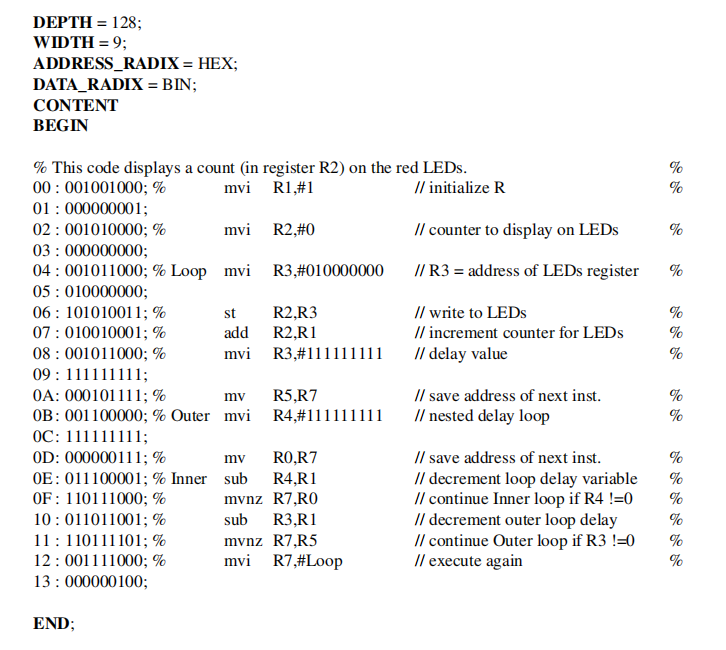
\includegraphics[scale = 0.65]{source/picture/Lab10/pic7.png}
    \caption{An example program in a memory initialization file (MIF)}
\end{figure}
\subsubsection{Simulation}
\begin{figure}[h]
    \centering
    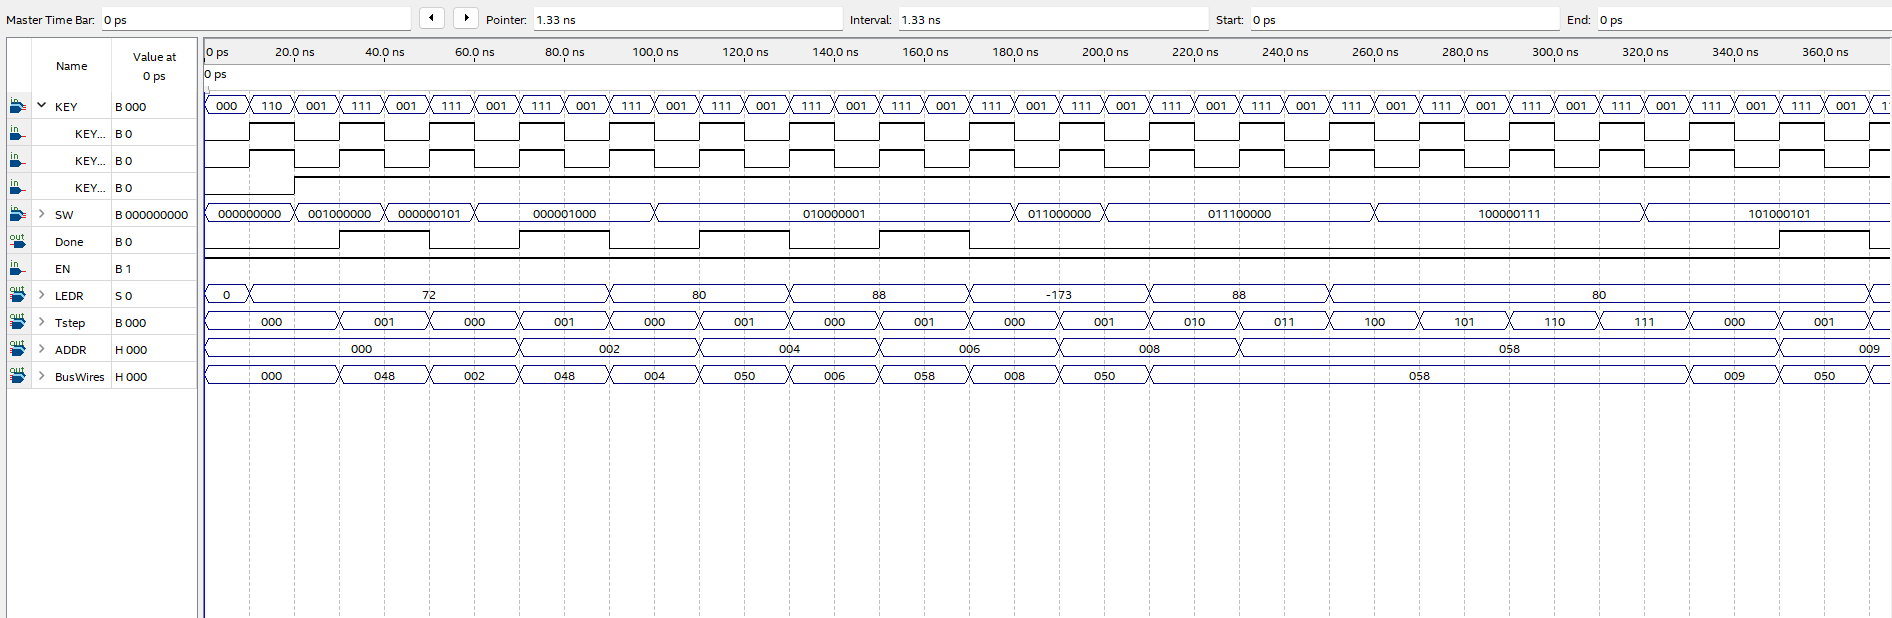
\includegraphics[scale = 0.3]{source/picture/Lab10/pic4.png}
    \caption{Simulation waveform}
\end{figure}
\begin{figure}[h]
    \centering
    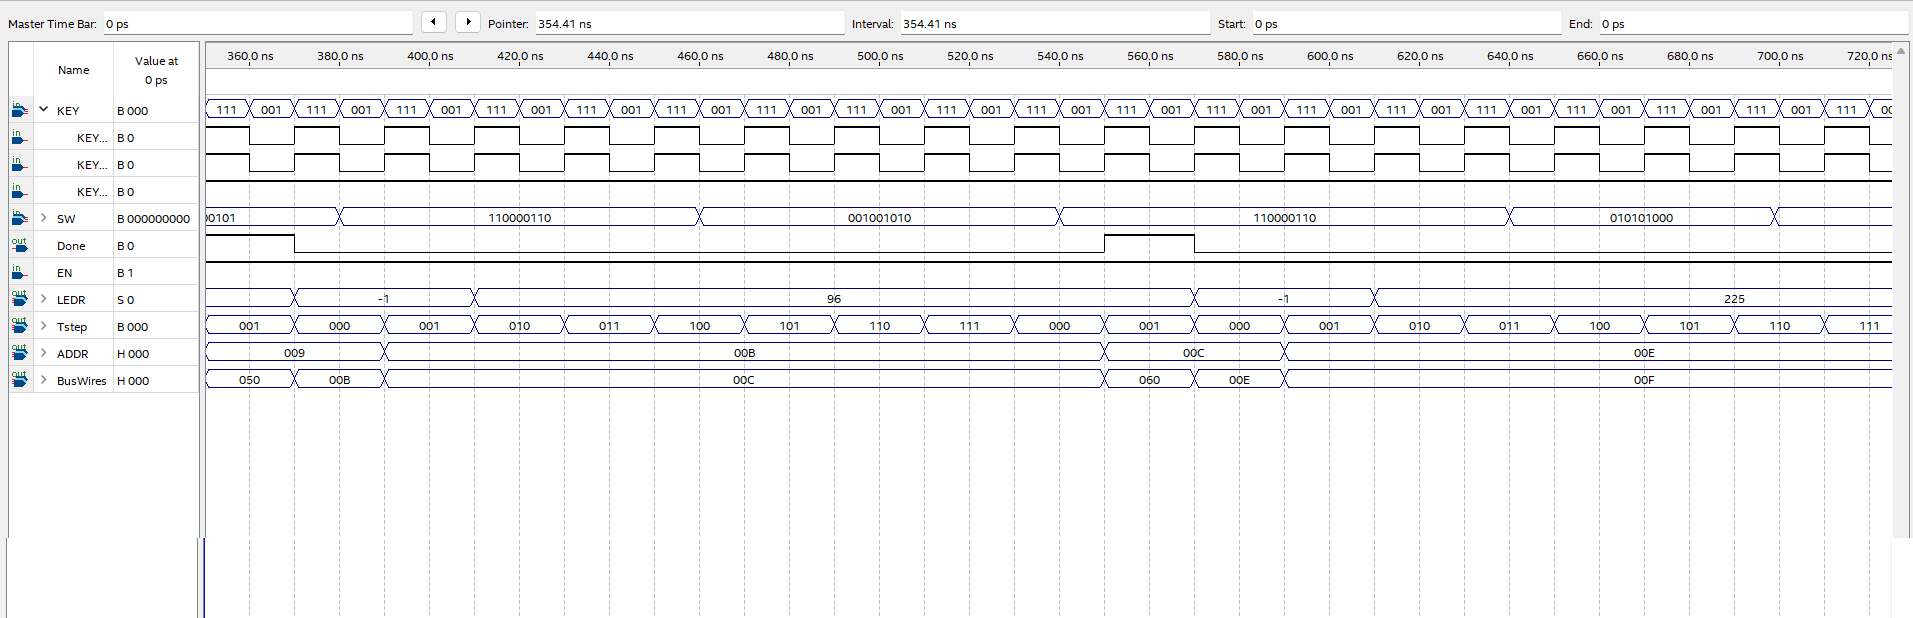
\includegraphics[scale = 0.3]{source/picture/Lab10/pic5.png}
    \caption{Simulation waveform}
\end{figure}
\begin{figure}[h]
    \centering
    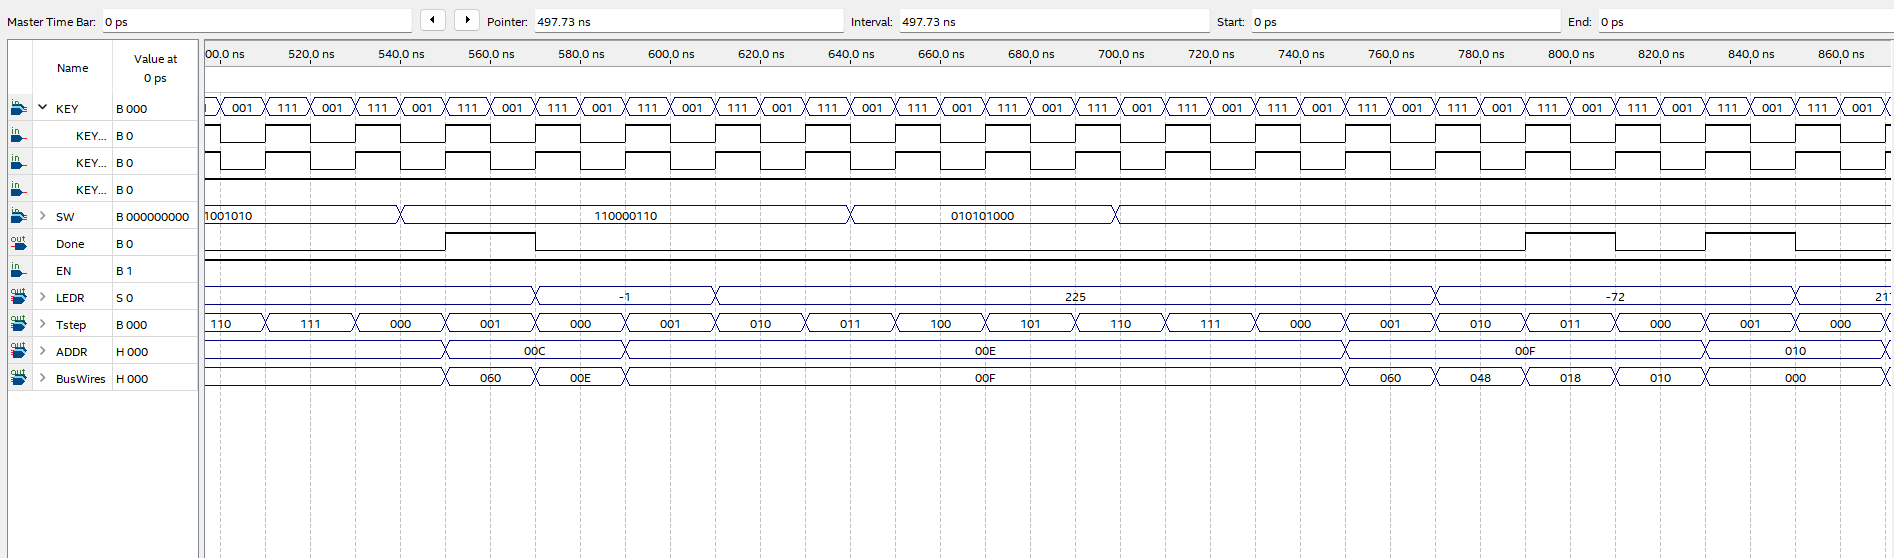
\includegraphics[scale = 0.3]{source/picture/Lab10/pic6.png}
    \caption{Simulation waveform}
\end{figure}
\newpage
\subsection{Explain waveform time}
\begin{itemize}
    \item \#0 Address is 000 and the next cycle (t = 30) when Posedge Clk LEDR display R1 = 72 as this is the mvi and it is store to R1, Buswire show the value R1 = 048 in hexa
    \item \#70 Address is 002 as it counter to display to the LEDR the value of R2 = 72 as this is the mvi of R2
    \item \#110 Address is 004 the next cycle (t = 130) and when then LEDR display R3 = 80 as this is the mvi, and R3 equal to Address of Led Register
    \item \#150 Address is 006 the next cycle (t = 170) At this time the processor storing st the value of R3 and R2
    \item \#190 Address is 008 and this is the increment of add R2 when it add and reach to 80, and when (t = 210) the Buswire start to delay until it reach at address 009. It delay the address of R3 = 058, and the value is 80
    \item \#230 Address is 058 the next cycle (t = 230) at this time the process is delaying value of R2
    \item \#350 Address is 009 the next cycle (t = 370) LEDR display -1
    \item \#390 Address is 00B  the next cycle (t = 410) LEDR display value of R4 and also delay value of R4
    \item \#550 Address is 00C the next cycle (t = 570) LEDR display -1
    \item \#590 Address is 00E the next cycle (t = 610) LEDR display the Inner sub of R4 and R1
    \item \#750 Address is 00F the next cycle (t = 770) LEDR continue Inner Loop R4
    \item The address 006, 00A and 00D, the value is store so the LED is not display this
\end{itemize}
